\documentclass{prova}

\usepackage{amsmath}
\usepackage{amsfonts}
\usepackage[export]{adjustbox}

\setlength{\textwidth}{18cm}
\setlength{\textheight}{27cm}
\setlength{\topmargin}{-2.3cm}
\setlength{\oddsidemargin}{-1cm}

\renewcommand{\sin}{\,\mbox{sen}\,}
\newcommand{\ds}{\displaystyle}

%\hyphenation{cor-res-pon-d\^en-ci-as}

\professor{Prof.\@ Adriano Barbosa}
\disciplina{C\'alculo de V\'arias Vari\'aveis}
\avaliacao{PS}
\curso{Matem\'atica}
\data{06/09/2023}

\begin{document}
	\cabecalho{5}  % o numero 5 indica a qnt de quadros na tabela de nota

    \textbf{Todas as respostas devem ser justificadas.}

    \vspace{0.5cm}
    \textbf{Avalia\c{c}\~ao P1:}
    \begin{questionario}
        \q{Esboce o maior dom\'{\i}nio das fun\c{c}\~oes:}
            \begin{questionario}
                \qq{$f(x,y) = \ln(1-x^2-y^2)$}
                \qq{$f(x,y) = \ds\frac{1}{x-y^2}$}
            \end{questionario}
        \q{Suponha $z=f(x,y)$, onde $x=g(s,t)$, $y=h(s,t)$, $g(1,2)=3$,
           $\ds\frac{\partial g}{\partial s}(1,2) = -1$, $\ds\frac{\partial
           g}{\partial t}(1,2) = 4$, $h(1,2) = 6$, $\ds\frac{\partial h}{\partial
           s}(1,2) = -5$, $\ds\frac{\partial h}{\partial t}(1,2) = 10$,
           $\ds\frac{\partial f}{\partial x}(3,6) = 7$ e $\ds\frac{\partial
           f}{\partial y}(3,6) = 8$. Determine o valor de $\ds\frac{\partial
           z}{\partial s}$ e $\ds\frac{\partial z}{\partial t}$ quando $s=1$ e
           $t=2$.}
        \q{A temperatura $T$ de um ponto $P$ numa bola de metal \'e inversamente
           proporcional \`a dist\^ancia de $P$ ao centro da bola, que tomamos como
           sendo a origem. A temperatura no ponto $(1,2,2)$ \'e de $120^{\circ}$C.
           Determine a taxa de varia\c{c}\~ao de $T$ em $(1,2,2)$ na dire\c{c}\~ao
           $(1,-1,1)$.}
        \q{Determine se as afirma\c{c}\~oes s\~ao verdadeiras ou falsas justificando.}
            \begin{questionario}
                \qq{Se $f$ tem um m\'{\i}nimo local em $(a,b)$ e $f$ \'e diferenci\'avel
                    em $(a,b)$, ent\~ao $\nabla f(a,b) = (0,0)$.}
                \qq{Se $f(x,y) = \ln{y}$, ent\~ao $\nabla f(x,y) =
                    \ds\frac{1}{y}$.}
            \end{questionario}
        \q{Determine os m\'aximos e m\'{\i}nimos de $f(x,y,z)=2x+2y+z$ restrita a
           $x^2+y^2+z^2=9$.}
    \end{questionario}

    \vspace{0.5cm}
    \textbf{Avalia\c{c}\~ao P2:}
    \begin{questionario}
        \q{Calcule a integral $\ds\iint_R x\sin(x+y)\ dA$, onde $R =
           [0,\pi/6]\times [0,\pi/3]$.}
        \q{Calcule a integral iterada invertendo a ordem de integra\c{c}\~ao
           $\ds\int_0^1 \int_x^1 \cos(y^2)\ dy\ dx$.}
        \newpage{}
        \q{Escreva $\ds\iint_R f(x,y)\ dA$ como uma integral iterada para cada uma
           das regi\~oes $R$ abaixo.}

            \begin{enumerate*}
                \item{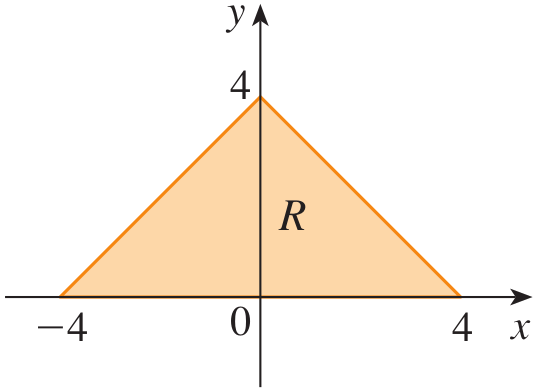
\includegraphics[width=0.3\textwidth,valign=t]{p2-q2-1.png}}
                \item{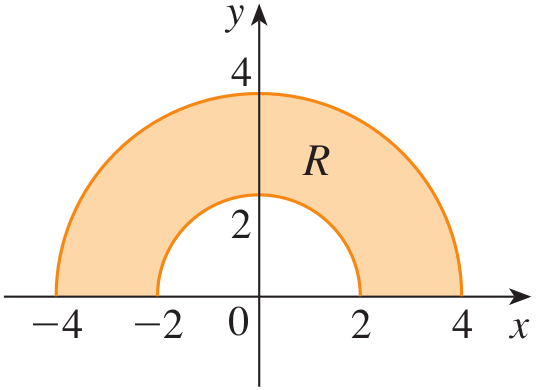
\includegraphics[width=0.3\textwidth,valign=t]{p2-q2-2.png}}
            \end{enumerate*}
        \q{}
            \begin{questionario}
                \qq{Escreva a integral tripla de uma fun\c{c}\~ao cont\'{\i}nua $f(x,y,z)$
                    sobre o s\'olido abaixo determinando seus limites de
                    integra\c{c}\~ao.}
                \qq{Calcule o volume do s\'olido utilizando a integral tripla
                    encontrada no item anterior.}
                \begin{figure}[h]
                    \centering
                    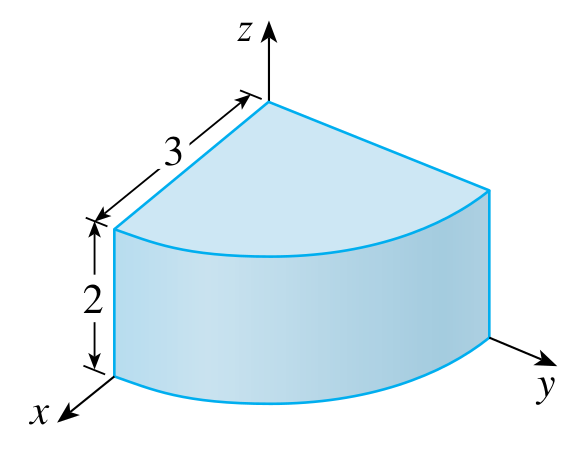
\includegraphics[width=0.3\textwidth]{p2-q4.png}
                \end{figure}
            \end{questionario}
        \q{Calcule $\ds\iiint_E x^2+y^2\ dV$, onde $E$ est\'a entre as esferas
           $x^2+y^2+z^2=4$ e $x^2+y^2+z^2=9$.}
    \end{questionario}
\end{document}
